\subsection{State of system}

The state of the system have to be reviewed from different perspectives. Code Climate provides the information seen in \autoref{fig:ccstate}.

\begin{figure}[H]
    \centering
    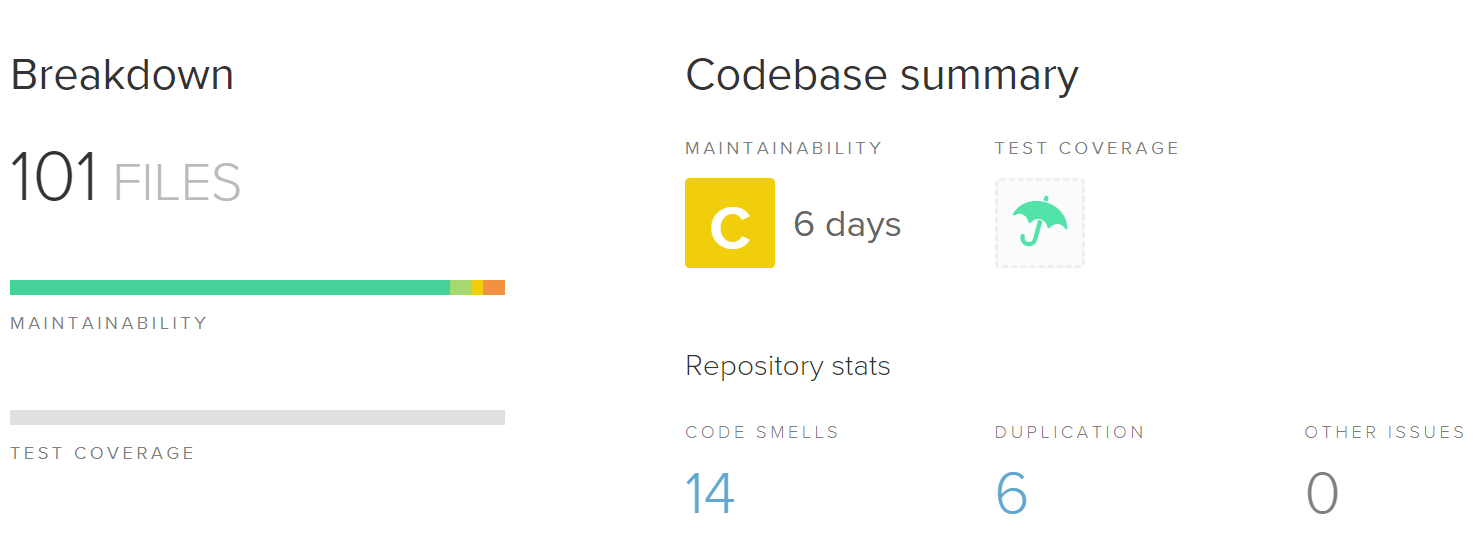
\includegraphics[width=\textwidth]{resources/CCstate.PNG}
    \caption{Codebase summary.}
    \label{fig:ccstate}
\end{figure}

Looking into these issues, many of them concern methods having too many lines of code. System limit is 25, while some happen to contain 40 lines of code. Some of the other smells revolve similar code blocks across different files. Essentially, these issues are categorized as either duplication or complexity.

SonarCloud is another integrated tool with some of the same properties as Code Climate. Taking a look on the summary reveals 36 code smells and a potential critical security issue. A summary of these can be seen below in \autoref{fig:scstate}.

\begin{figure}[H]
    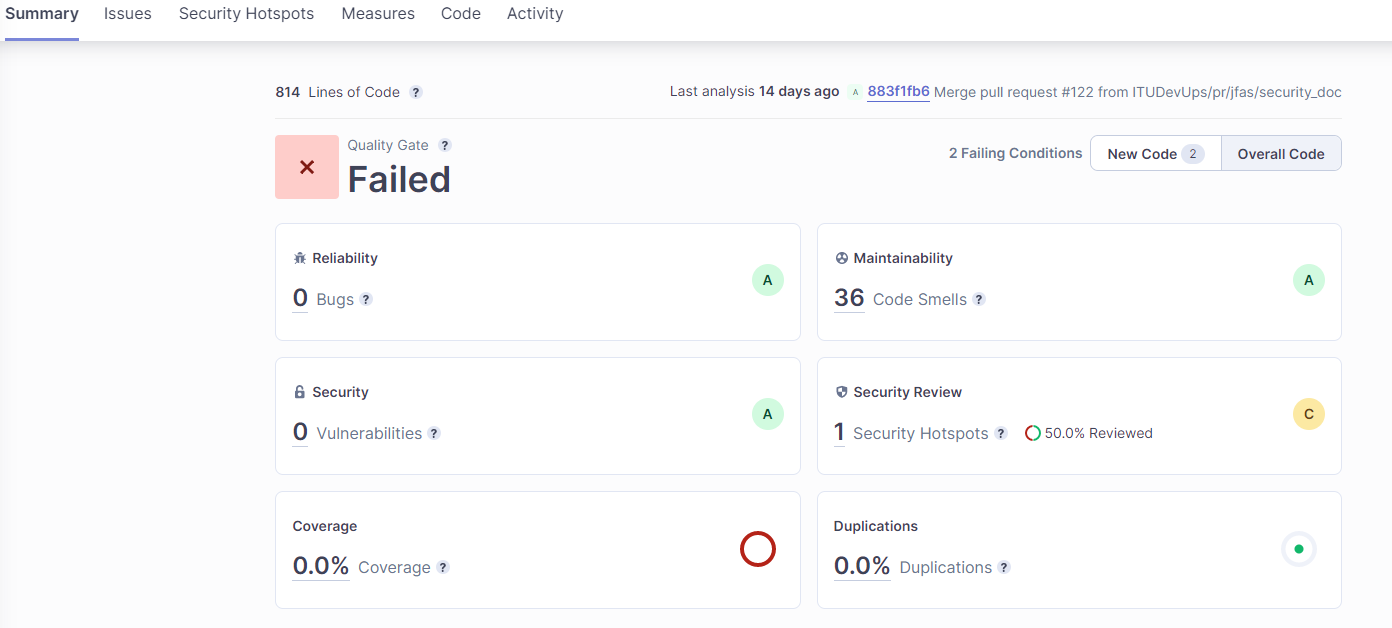
\includegraphics[width=\textwidth]{resources/sonarcloud2.PNG}
    \caption{SonarCloud summary.}
    \label{fig:scstate}
\end{figure}

It provides a deep look into the code smells giving an overview over severity, location, status and if it is assigned to a team member. A view of this can be seen in \autoref{fig:sccodesmells}.

\begin{figure}[H]
    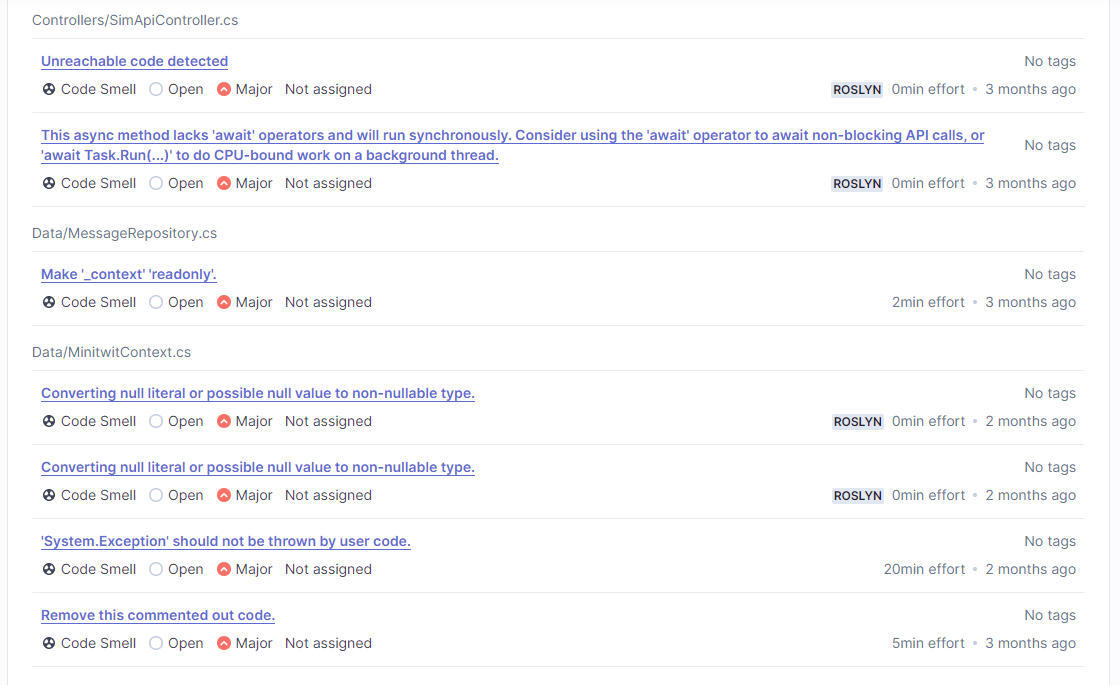
\includegraphics[width=\textwidth]{resources/sonarclouddeep}
    \caption{SonarCloud code smells.}
    \label{fig:sccodesmells}
\end{figure}

Generally, the issues are related to clean code properties such as style, quality, maintainability and design - which in large part is handled by SonarClouds Roslyn\footnote{Roslyn is the codename for the .NET Compiler Platform, used for compiling and understanding C\# code.} integration. The issues in the snippet are the most occurring detections found by SonarCloud at the moment.

The security issue detected in SonarCloud is from the backend-file appsettings.json, where a hardcoded password for digital ocean db-connection is present. The solution would be to tokenize this password as has been done with other repository secrets. SonarCloud does not approve the current state of the program to be deployed to production. These issues are likely from the time before the SonarCloud integration to the CI-pipeline, as a new pull request with these would not have passed the checks in GitHub Actions.

As it is viewable in the two tools, SonarCloud and Code Climate, the overlap of what they have found is not huge. The reports created from both provides a deeper knowledge of MiniTwit and how it can be strengthened in the refactoring phase and mitigated during pull requests. In short, Code Climate excels in eliminating technical debt and SonarCloud excels in ensuring software quality. 